\documentclass[12pt,a4paper]{article}

% Packages
\usepackage[utf8]{inputenc}    % Encoding
\usepackage[T1]{fontenc}       % Font encoding
\usepackage{lipsum}            % Dummy text (optional)
\usepackage{amsmath, amssymb}  % Math symbols
\usepackage{graphicx}          % For images
\usepackage{hyperref}          % Clickable links
\usepackage{enumitem}
\usepackage[a4paper, top=2cm, bottom=2cm, left=2cm, right=2cm]{geometry} % the margins
\usepackage{tabularx}


% Title info
\title{RDFIA Reports: tp 1, 2 and 3}
\author{Titouan Guerin \& Yacine Chettab}
\begin{document}
\date{\today}
\maketitle

\section{Theoretical foundation}

\subsection{Supervised Dataset}

\paragraph{Questions} 

\begin{enumerate}
    \item \textbf{$\star$ What are the train, val and test sets used for?} \newline
    The train set is used to train the model, 
    the validation set is used to tune the hyperparameters during the training of the model, 
    and the test set is used to evaluate the model's performance 
    (data that is not in the train set, so not seen by the model previously).

    \item \textbf{What is the influence of the number of examples $N$?} \newline
    The number of examples $N$ influences the model's ability to generalize, which means that by seeing
    enough examples, the model can learn to make predictions on unseen data. On the other hand, if 
    $N$ is too little, then the model will do more of a memorization of the training data, so it does not
    actually learn to generalize the problem. However, having too many samples $N$ can be a problem in terms 
    of training time and computational resources.
\end{enumerate}

\subsection{Network Architecture (forward)}

\paragraph{Questions}

\begin{enumerate}[resume]
    \item \textbf{Why is it important to add activation functions between linear transformations?} \newline
    Having no activation functions between the linear layers would make the whole network linear 
    (which is not what we are looking for). Chaining linear transformations is the same as having one linear
    layer but with just more weights. So the activation functions allow the network to learn non-linear
    patterns in the data.

    \item \textbf{$\star$ What are the sizes $n_x$, $n_h$, $n_y$ in the figure 1? In practice, how are these sizes chosen?}
    \begin{itemize}
        \item $n_x$ is the size of the input layer, the number of features for one data point,
        \item $n_h$ is the size of the hidden layer, a hyperparameter that is determined before training,
        \item $n_y$ is the size of the output layer, the number of classes for classification problems.
    \end{itemize}

    \item \textbf{What do the vectors $\hat{y}$ and $y$ represent? What is the difference between these two quantities?} \newline
    The vector $\hat{y}$ represents the predicted output of the model, while $y$ represents the true labels.

    \item \textbf{Why use a SoftMax function as the output activation function?} \newline
    The SoftMax function maps the output of the neural network to a probability distribution.
    This means that all the values outputted by the model are mapped between 0 and 1, and the sum
    of all the values are equal to 1: $\sum_{i=1}^{n} \hat{y}_i = 1$.

    \item \textbf{Write the mathematical equations allowing to perform the forward pass of the neural network, i.e.
allowing to successively produce $\tilde{h}$, $h$, $\tilde{y}$ and $\hat{y}$ starting at $x$.} 
    \begin{itemize}
        \item $\tilde{h} = W_h x + b_h$
        \item $h = \text{ReLU}(\tilde{h})$
        \item $\tilde{y} = W_y h + b_y$
        \item $\hat{y} = \text{SoftMax}(\tilde{y})$
    \end{itemize}
\end{enumerate}

\subsection{loss function}

\paragraph{Questions}

\begin{enumerate}[resume]
    \item \textbf{During training, we try to minimize the loss function. For cross entropy and squared error, how must
the $\hat{y}_i$ vary to decrease the global loss function $\mathcal{L}$?} \newline
    For the MSE, the prediction $\hat{y}$ is compared directly to $y$, so to minimize the loss, 
    we want the difference between those two values to be as small as possible. In this case we work 
    with real numerical values. This loss works for both regression and classification problems. \newline
    On the other hand, for the cross-entropy, we are working exclusively with probabilities, so to minimize the loss,
    we want the predicted probability $\hat{y}_i$ of the true class to be as close to 1 as possible,
    (and the predicted probabilities of the other classes to be as close to 0 as possible). Here $y$ is just a 
    probability vector, with just zeros except for the true class which is 1.

    \item \textbf{How are these functions better suited to classification or regression tasks?} \newline
    MSE is naturally suited to regression, since its gradient is linear in the prediction error, 
    providing a good measure of how far the prediction is from the target. 
    However, in classification this linear behavior is less effective, because it does not 
    properly penalize cases where the model is very confident but wrong (not enough at least).  

    Cross-entropy, on the other hand, has a gradient that grows rapidly 
    when the predicted probability for the correct class is small. 
    Basically you want to penalize a confident but wrong prediction because it impacts the other predicted probabilities.
    Since the penalty (or cost) of CE is logarithmic, and hence more harsh on wrong predictions,
    the gradient of the loss is larger and allows the model to learn faster.

    \begin{figure}[h]
        \centering
        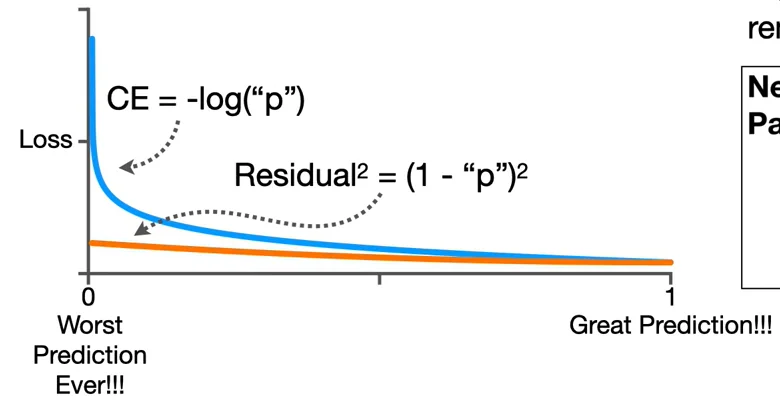
\includegraphics[width=0.4\textwidth]{CEillustration.png}
        \caption{\protect\href{https://www.reddit.com/r/learnmachinelearning/comments/yyfhm4/understanding_statquest_video_why_cross_entropy/}{Cross-Entropy vs MSE derivative comparison.}}
        \label{fig:ce_vs_mse}
    \end{figure}

\end{enumerate}

\subsection{Optimization algorithm}

\paragraph{Questions}

\begin{enumerate}[resume]
    \item \textbf{What seem to be the advantages and disadvantages of the various variants of gradient descent
                between the classic, mini-batch stochastic and online stochastic versions? Which one seems the most
                reasonable to use in the general case?} 
    \begin{tabularx}{0.9\textwidth}{l X X}
        \hline
        \textbf{Method} & \textbf{Advantages} & \textbf{Disadvantages} \\ \hline
        Batch GD & Stable convergence, accurate gradients & High memory usage, slow \& expensive for large datasets, possible local minimum \\ \hline
        Mini-batch SGD & faster convergence, no local minima, better 'exploration' of the dataset & batch size tuning, noise \\ \hline
        Online SGD & Fast updates, low memory usage & Noisy gradients, less stable convergence \\ \hline
    \end{tabularx} \newline
    \newline
    Overall it is pretty safe to conclude that Mini-batch SGD is the most reasonable method to use in the general case,
    because it essentially is a mix of the two other methods: faster convergence and lower computational cost.

    \item \textbf{$\star$ What is the influence of the learning rate $\eta$ on learning?} \newline
    Recap: the learning rate $\eta$ is a hyperparameter that controls how strongly the weights are updated during training. \newline
    A high learning rate means that the weights are updated strongly at each training step, which can lead to fast convergence but also 
    to the overshooting of the optimal solution. Overshooting means that the model will diverge, or jump around the optimal solution without actually reaching it. \newline
    On the contrary, a low learning rate means that each update step changes the weights only slightly, which can lead to slow convergence.
    This can be helpful to explore the local minima, but can also lead to getting stuck there. \newline
    To address these drawbacks, one good technique is to change $\eta$ over time. By starting with a high learning rate, and then
    decreasing it as we get closer to the optimal solution (over time), we allow the model to make bigger steps at the beginning of the training, 
    and to then make smaller careful steps when we are close to the optimal solution.

    \item \textbf{$\star$ Compare the complexity (depending on the number of layers in the network) of calculating the
            gradients of the loss with respect to the parameters, using the naive approach and the backprop algorithm} \newline
    For the naive approach, the gradient of the loss is calculated for each parameter independently. 
    For example, for the weights of the second layer, we would calculate the gradient of the loss with respect to each weight $w_{ij}$ in 
    the weight matrix $W_2$. And for the gradients of the first layer, we would re-calculate the gradients of the second layer, 
    and then compute the gradients with respect to the first layer. Even for a two-layer network, we can see that this approach is very computationally 
    expensive, since we keep calculating the same gradients over and over. \newline
    With the backpropagation algorithm, each gradient is calculated only once. If we take our previous example with only two layers, 
    after calculating the gradients of the second layer, we keep those gradients in memory and use them to calculate the gradients of the first layer. 
    In essence, this means that all of the gradients are calculated in a single backward pass, 
    without having to recompute the gradients of the loss like in the naive method. \newline
    This backpropagation algorithm is much more efficient and becomes mandatory for deep networks with many layers. \newline
    Remark on the $\mathcal{O}$ complexity: \newline
    For a network with $L$ layers, let $n_l$ be the number of parameters in layer $l$.  

    \begin{itemize}
        \item computing $\frac{\partial \mathcal{L}}{\partial W_l}$ for each layer separately (naive):  
        \[
        \mathcal{O}\Big(\sum_{l=1}^L \sum_{k=l}^L n_k\Big) = n \Big(\sum_{l=1}^{L} (L - l + 1)) = n(1 + 2 + \text{\dots} + L) = n \frac{L(L+1)}{2}
        \sim \mathcal{O}(L^2 \cdot n_\text{avg})
        \]  
        where $n_\text{avg}$ is the average number of parameters per layer.  

        \item For the backpropagation algorithm:  
        \[
        \mathcal{O}\Big(\sum_{l=1}^L n_l\Big) = n + n + \text{\dots} + n = L \cdot n  = \sim \mathcal{O}(L \cdot n_\text{avg})
        \]  
    \end{itemize}

    \item \textbf{What criteria must the network architecture meet to allow such an optimization procedure ?} \newline
    Each layer (linear, activation, cost $\dots$) must be differentiable in order for the backpropagation to be possible.
    There also needs to be some form of memory to save every input and output of each layer during the forward pass as they are
    needed for the backward pass. Finally, the gradients produced must not be either extremely small or large, as they would break 
    the backpropagation (vanishing or exploding gradients).

    \item \textbf{The function SoftMax and the loss of cross-entropy are often used together and their gradient is very simple. Show that the loss can be simplified by:
    $$ l = - \sum_{i}y_i \tilde{y}_i + \log (\sum_{i} e^{\bar{y}_i}) $$} \newline
    Recap: we write the cross-entropy loss as:
    \[
    l = - \sum_{i} y_i \log(\hat{y}_i)
    \]
    Here $\hat{y}_i$ is the output of the SoftMax function, so we can replace it in the loss:
    \begin{align*}
    l &= - \sum_{i} y_i \log\Big(\frac{e^{\tilde{y}_i}}{\sum_{j} e^{\tilde{y}_j}}\Big) \\
    l &= - \sum_{i} y_i \Big(\log(e^{\tilde{y}_i}) - \log(\sum_{j} e^{\tilde{y}_j})\Big) \\
    l &= - \sum_{i} y_i \Big(\tilde{y}_j - \log(\sum_{j} e^{\tilde{y}_j})\Big) \\
    l &= - \sum_{i} y_i \tilde{y}_i + \sum_{i} y_i \log(\sum_{j} e^{\tilde{y}_j}) \\
    \end{align*}
    Since $y$ is the label vector, composed of zeros except for the true class which is 1, then we know that the sum of all the $y_i$ is equal to 1, so:
    \[
    l = - \sum_{i} y_i \tilde{y}_i + \log(\sum_{j} e^{\tilde{y}_j})
    \]

    \item \textbf{Write the gradient of the loss (cross-entropy ) relative to the intermediate outputs $\tilde{y}$:
    $$ \frac{\partial l}{\partial \tilde{y}_i} = \dots \implies \nabla_{\bar{y}} l =  
    \begin{bmatrix}
    \frac{\partial \ell}{\partial \tilde{y}_1} \\
    \vdots \\
    \frac{\partial \ell}{\partial \tilde{y}_n}
    \end{bmatrix}
    = \dots$$} \newline
    % Reminder: \[ \sum_{i} y_i = 1 \]
    We are trying to find:
    \begin{align*}
        \frac{\partial l}{\partial \tilde{y}_i} = \sum_{k} \frac{\partial l}{\partial \hat{y}_k}  \frac{\partial \hat{y}_k}{\partial \tilde{y}_i}
    \end{align*}
    We need to compute $ \frac{\partial l}{\partial \hat{y}_k} $:
    \begin{align*}
        \frac{\partial l}{\partial \hat{y}_k} &= \frac{\partial}{\partial \hat{y}_k} \Big(- \sum_{k} y_k \log(\hat{y}_k)\Big) \\
        &= - y_k \frac{\partial}{\partial \hat{y}_k} (\log(\hat{y}_k)) \\
        &= - y_k \frac{1}{\hat{y}_k} \\
        &= - \frac{y_k}{\hat{y}_k}
    \end{align*}
    Next we compute $ \frac{\partial \hat{y}_k}{\partial \tilde{y}_i} $, which is the derivative of the SoftMax function
    (the explanation was taken from this \href{https://eli.thegreenplace.net/2016/the-softmax-function-and-its-derivative/}{source}).
    The derivative has two cases, when $i = k$ and when $i \neq k$, which are:
    \[
        \frac{\partial \hat{y}_i}{\partial \tilde{y}_i} = \hat{y}_i (1 - \hat{y}_i) \quad \text{and} \quad
        \frac{\partial \hat{y}_k}{\partial \tilde{y}_i} = - \hat{y}_i \hat{y}_k 
    \]
    So if we combine all of this:
    \begin{align*}
        \frac{\partial \ell}{\partial \tilde{y}_i} 
        &= \sum_{k=i} \Big(- \frac{y_k}{\hat{y}_k} \cdot \hat{y}_i (1 - \hat{y}_k) \Big)
        + \sum_{k \neq i} \Big(- \frac{y_k}{\hat{y}_k} \cdot \hat{y}_i (0 - \hat{y}_k) \Big) \\
        &= \sum_{k=i} \Big(- y_i \frac{\hat{y}_i (1 - \hat{y}_i)}{\hat{y}_i} \Big)
        + \sum_{k \neq i} \Big(- y_k \frac{\hat{y}_i (- \hat{y}_k)}{\hat{y}_k} \Big) \tag{1}\\
        &= \sum_{k=i} \Big(- y_i (1 - \hat{y}_i) \Big)
        + \sum_{k \neq i} \Big(y_k \hat{y}_i \Big) \\
        &= -y_i (1 - \hat{y}_i) + \sum_{k \neq i} y_k \hat{y}_i \\
        &= -y_i + y_i \hat{y}_i + \hat{y}_i \sum_{k \neq i} y_k \\
        &= -y_i + y_i \hat{y}_i + \hat{y}_i (1 - y_i) \\[1mm]
        &= \hat{y}_i - y_i
    \end{align*}

    In terms of matrices, the gradient of the loss than simply be expressed as: 
    $$\nabla_{\bar{y}} l =  
    \begin{bmatrix}
    \frac{\partial \ell}{\partial \tilde{y}_1} \\
    \vdots \\
    \frac{\partial \ell}{\partial \tilde{y}_n}
    \end{bmatrix}
    = \hat{y} - y$$

    Note: at the equation (1), we change the index from k to i for the term where k=i. 
    This is because the sum only includes the case k=i, so k is effectively fixed to i. 
    All other terms do not appear in this sum. 
    This simplification allows us to replace k with i and remove the index from the expression.

    \item \textbf{Using backpropagation, write the gradient of the loss with respect to the weights of the output 
    layer $\mathbf{W}_y$. Note that computing this gradient uses $\nabla_{\tilde{\mathbf{y}}} \ell$. Do the same for $\mathbf{b}_y$.} \newline
    \[
    \frac{\partial \ell}{\partial W_{y,ij}} 
    = \sum_k \frac{\partial \ell}{\partial \tilde{y}_k} \frac{\partial \tilde{y}_k}{\partial W_{y,ij}}
    = \dots 
    \quad \implies \quad
    \nabla_{\mathbf{W}_y} \ell =
    \begin{bmatrix}
    \frac{\partial \ell}{\partial W_{y,11}} & \dots & \frac{\partial \ell}{\partial W_{y,1n_h}} \\
    \vdots & \ddots & \vdots \\
    \frac{\partial \ell}{\partial W_{y,n_y1}} & \dots & \frac{\partial \ell}{\partial W_{y,n_y n_h}}
    \end{bmatrix}
    = \dots
    \]

    So first of all,
    \[
    \tilde{y} = W_y h + b_y \quad \text{with} \quad h \in \mathbb{R}^{n_h}
    \]
    then by defining,
    \[
    \tilde{y}_k = \sum_{j=1}^{n_h} W_{y,ij}\,h_j + b_{y,k} ,
    \]

    We will now be able to simplify $ \frac{\partial \tilde{y}_k}{\partial W_{y,ij}} $ :
    
    \[
    \frac{\partial \ell}{\partial W_{y,ij}}
    = \sum_{k=1}^{n_y} \frac{\partial \ell}{\partial \tilde{y}_k}\,\frac{\partial \tilde{y}_k}{\partial W_{y,ij}}
    = \frac{\partial \ell}{\partial \tilde{y}_i}\,h_j 
    \]

    In matrix form:
    \[
    \nabla_{\mathbf{W}_y}\ell =
    \begin{bmatrix}
    \frac{\partial \ell}{\partial \tilde{y}_1} h_1 & \cdots & \frac{\partial \ell}{\partial \tilde{y}_1} h_{n_h}\\
    \vdots & \ddots & \vdots\\
    \frac{\partial \ell}{\partial \tilde{y}_{n_y}} h_1 & \cdots & \frac{\partial \ell}{\partial \tilde{y}_{n_y}} h_{n_h}
    \end{bmatrix}
    = \big(\nabla_{\tilde{\mathbf{y}}}\ell\big)\,\mathbf{h}^{\!\top}
    \]
    This means that the gradient of the weights is obtained by multiplying the loss gradient with the output of the hidden layer

    For the biases $b_y$:
    \[
    \frac{\partial \ell}{\partial b_{y,i}}
    = \sum_{k=1}^{n_y} \frac{\partial \ell}{\partial \tilde{y}_k}\,\frac{\partial \tilde{y}_k}{\partial b_{y,i}}
    = \frac{\partial \ell}{\partial \tilde{y}_i}
    \]
    so in vector form
    \[
    \nabla_{\mathbf{b}_y}\ell = \nabla_{\tilde{\mathbf{y}}}\ell .
    \]

    \item \textbf{$\star$ Compute the gradients: $\nabla_{\tilde{h}}\ell, \nabla_{W_h}\ell, \nabla_{b_h}\ell$}

    \begin{enumerate}
        \item \[ 
        \nabla_{\tilde{h}_i}\ell = \frac{\partial \ell}{\partial \tilde{h}_i}  
        = \sum_{k} \frac{\partial \ell}{\partial h_k} \frac{\partial h_k}{\partial \tilde{h}_i}
        \]
        For $h$ and $\tilde{h}$, the activation function is now $\tanh$. So:
        \[
        \frac{\partial h_k}{\partial \tilde{h}_i} = \frac{\partial \tanh(\tilde{h}_k)}{\partial \tilde{h}_i}
        \]
        Similarly to the case with Softmax, here the derivative of $\tanh$ only exists when $k=i$. And the derivative
        of $tanh(x)$ is: $1 - \tanh^2(x)$.
        So now we can replace with $\tilde{h}_k$:
        \[
        \frac{\partial h_k}{\partial \tilde{h}_i}
        = \frac{\partial \tanh(\tilde{h}_k)}{\partial \tilde{h}_i} \tag{1}
        = (1 - \tanh^2(\tilde{h}_i))
        = 1 - h_i^2
        \]
        Note: In (1), if we refer back to the figure of our neural network, we see that $h_i = \tanh(\tilde{h}_i)$, so $\tanh^2(\tilde{h}_i) = h_i^2$, 
        and like earlier since this equality only exists when $i=k$ then we can change the index 
        from $\tilde{h}_k$ to $\tilde{h}_i$ \newline
        So,
        \[
        \frac{\partial \ell}{\partial \tilde{h}_i}
        = \sum_k \frac{\partial \ell}{\partial h_k} \frac{\partial h_k}{\partial \tilde{h}_i}
        \]

        so since $\frac{\partial h_k}{\partial \tilde{h}_i}$ is nonzero only when $k = i$, the sum reduces to a single term:
        \[
        \frac{\partial \ell}{\partial \tilde{h}_i}
        = \frac{\partial \ell}{\partial h_i} \cdot (1 - h_i^2) 
        = \nabla_{\mathbf{h}}\ell \cdot (1 - h_i^2) 
        \]

        to develop this form a bit more, we can express $\frac{\partial \ell}{\partial h_i}$ as:
        \[
        \frac{\partial \ell}{\partial h_i} = \sum_j \frac{\partial \ell}{\partial \hat{y}_j} \frac{\partial \hat{y}_j}{\partial h_i}
        = \sum_j \delta_{j}^{(y)} W_{j,i}^{(y)} 
        \]
        with $\delta_{j}^{(y)} = \frac{\partial \ell}{\partial \tilde{y}_j}$

        and if we plug it back into the gradient of $\tilde{h}_i$, we obtain:
        \[
        \frac{\partial \ell}{\partial \tilde{h}_i} 
        = (1 - h_i^2) \frac{\partial \ell}{\partial h_i}
        = (1 - h_i^2) \sum_j \delta_{j}^{(y)} W_{j,i}^{(y)}
        \]
        which we can also write in vector form as:
        \[
        \nabla_{\tilde{\mathbf{h}}}\ell 
        = (1 - \mathbf{h}^2) \cdot \left( (W^{(y)})^\top \boldsymbol{\delta}^{(y)} \right)
        \]
        
        \item $\nabla_{W_h}\ell$ \newline 
        Recall,
        \[
        \delta^{(h)}_i \equiv \frac{\partial \ell}{\partial \tilde{h}_i}
        = (1-h_i^2)\,\frac{\partial \ell}{\partial h_i}.
        \]
        for one weight \(W^{(h)}_{i j}\), we have,
        \[
        \frac{\partial \ell}{\partial W^{(h)}_{i j}}
        = \frac{\partial \ell}{\partial \tilde{h}_i}\,\frac{\partial \tilde{h}_i}{\partial W^{(h)}_{i j}}.
        \]
        and ecause \(\tilde{h}_i = \sum_{j} W^{(h)}_{i j} x_j + b^{(h)}_i\), we have $\frac{\partial \tilde{h}_i}{\partial W^{(h)}_{i j}} = x_j$, we arrive at:
        \[
        \frac{\partial \ell}{\partial W^{(h)}_{i j}} = \delta^{(h)}_i x_j
        \]
        This shows each weight-gradient is the product of the corresponding hidden delta and the input value that feeds that weight.

        
        \item $\nabla_{b_h}\ell$ \newline
        each bias \(b^{(h)}_i\) affects only its input of the activation function \(\tilde{h}_i\), so:
        \[
        \frac{\partial \ell}{\partial b^{(h)}_i}
        = \frac{\partial \ell}{\partial \tilde{h}_i}\,\frac{\partial \tilde{h}_i}{\partial b^{(h)}_i}.
        \]
        and we know that the second partial is equal to 1 because of the form of $\tilde{h}_i$ (see previous questions), we can write it as:
        \[
        \frac{\partial \ell}{\partial b^{(h)}_i} = \delta^{(h)}_i = \nabla_{\tilde{h}}\ell
        \]
        Note: $\delta^{(h)}_i = \frac{\partial \ell}{\partial \tilde{h}_i}$ is the same as for the previous questions
        
    \end{enumerate}

\end{enumerate}

\end{document}